\section{Задание 5. Поток векторного поля}

\textbf{Условие.}

\begin{multicols}{2}
    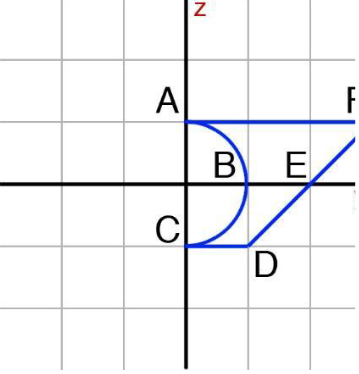
\includegraphics[height=7cm]{images/5a1}

    Дано тело $T$, ограниченное следующими поверхностями: $\displaystyle y - \sqrt{1 - x^2 - z^2} = 0, x^2 + z^2 = 1, y - z = 2$.

    На рисунке представлено сечение тела $T$ координатной плоскостью $Oyz$.

    1) Изобразите тело $T$ на графике в пространстве.

    2) Вычислите поток поля

    $\displaystyle \overrightarrow{a} = (\cos^2(z + y))\overrightarrow{i} + 2x\overrightarrow{j} + \left(\sqrt{y + 5} + 2z\right) \overrightarrow{k}$

    через боковую поверхность тела $T$, образованную вращением дуги $ABC$ вокруг оси Oy, в направлении внешней нормали поверхности тела $T$.
\end{multicols}


\vspace{10mm}
\textbf{Решение.}

\begin{enumerate}
	\item Графики:

        		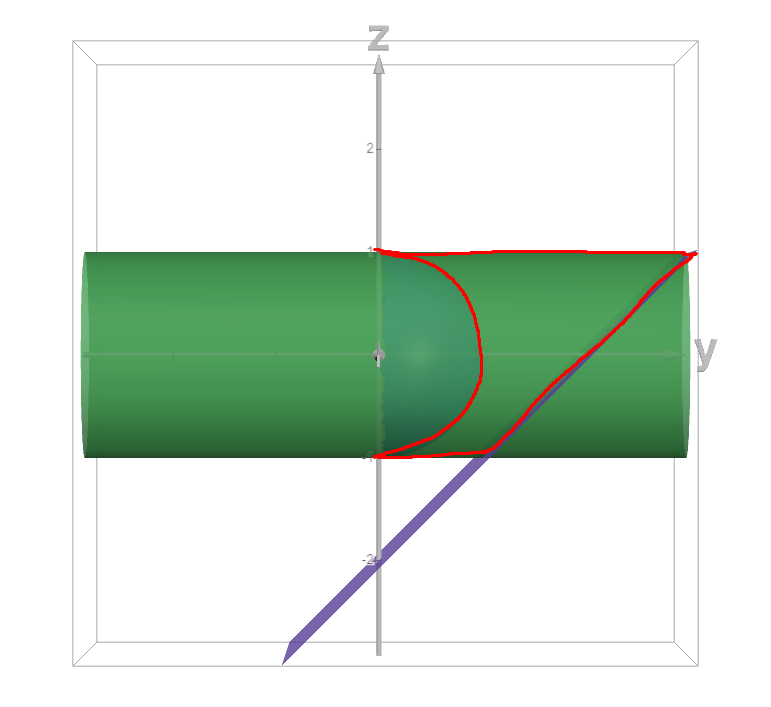
\includegraphics[height=80mm]{images/5_1a}
		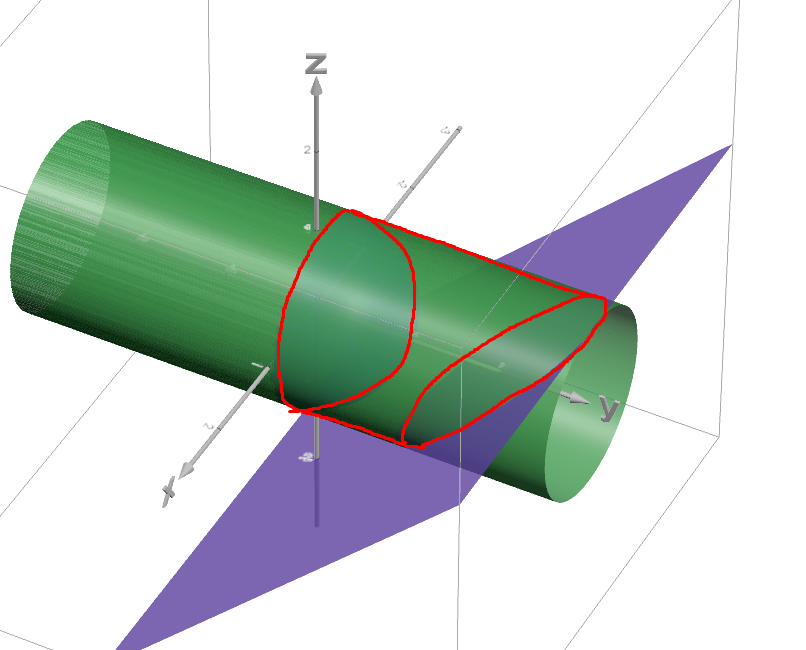
\includegraphics[height=80mm]{images/5_1b}

	\item Векторное поле: $\overrightarrow{a} = (\cos^2(z + y))\overrightarrow{i} + 2x\overrightarrow{j} + \left(\sqrt{y + 5} + 2z\right) \overrightarrow{k}$, поверхность задается уравнением: $y - \sqrt{1 - x^2 - z^2} = 0$.\\
Потоком векторного поля через эту поверхность будет двойной интеграл: ${\displaystyle \iint_\sigma} \cos^2(z+y)\hspace{1mm}dy dz + 2x\hspace{1mm}dx dz + (\sqrt{y + 5} + 2x)\hspace{1mm}dx dy$. Разобъем на три интеграла: ${\displaystyle \iint_{D_1}} \cos^2(z+y)\hspace{1mm}dy dz + {\displaystyle \iint_{D_2}}2x\hspace{1mm}dx dz + {\displaystyle \iint_{D_3}}(\sqrt{y + 5} + 2x)\hspace{1mm}dx dy$. $D_1 = \begin{cases} y \geqslant 0 \\ z \leqslant \sqrt{1 - y^2} \end{cases}; \hspace{2mm} D_2 =  x^2 + z^2 \leqslant 0; \hspace{2mm} D_3 = \begin{cases} y \geqslant 0 \\ y \leqslant \sqrt{1 - x^2} \end{cases}\\$

Так как поток идет в направлении внешнего вектора нормали, то интегрировать мы будем в этом направлении для плоскости $0yz$ и аналогично для остальных:

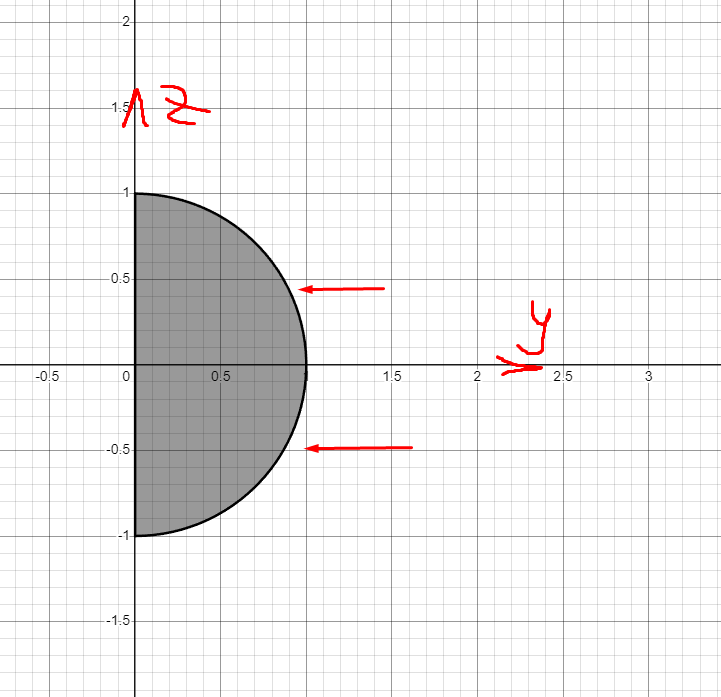
\includegraphics[height=80mm]{images/5_2}


${\displaystyle\iint_{D_1}}\cos^2(z + y) ={\displaystyle \int_{-1}^{1}}\int_{z = \sqrt{1 - y^2}}^{z = 0} \cos^2(y + z) \hspace{1mm} dy dz = {\displaystyle \int_{-1}^{1}}\int_{z = \sqrt{1 - y^2}}^{z = 0} \frac{1 +\cos(2y + 2z)}{2} \hspace{1mm} dy dz = {\displaystyle \int_{-1}^{1}\frac{1}{2}} ((0 - \sqrt{1 - y^2}) + \int_{z = \sqrt{1 - y^2}}^{z = 0} \cos(2y + 2z)) \hspace{1mm} dz) dy = {\displaystyle \frac{1}{2}\int_{-1}^{1}} (-\sqrt{1 - y^2} + {\displaystyle \frac{1}{2}}(\sin 2y - \sin(2\sqrt{1 + y^2} + 2y))) dy \approx-1\\$

${\displaystyle \iint_{D_2}}2x \hspace{1mm}dxdz = {\displaystyle \int_{-1}^{1}}\int_{z = -\sqrt{1 - x^2}}^{z = \sqrt{1 - x^2}}2x \hspace{1mm} dx dz = {\displaystyle \int_{-1}^{1}}4x\sqrt{1 - x^2} \hspace{1mm} dx= {\displaystyle \int_{-1}^{1}}2\sqrt{1 - x^2} \hspace{1mm} dx^2 = 0\\$

${\displaystyle \iint_{D_3}}(\sqrt{y  +5} + 2x )\hspace{1mm} dxdy = {\displaystyle \int_{-1}^{1}}\int_{y = \sqrt{1 - x^2}}^{y = 0}(\sqrt{y + 5} + 2x) \hspace{1mm} dx dy = {\displaystyle \int_{-1}^{1}}(-\frac{2}{3}(5\sqrt{5} - \sqrt{(5 + \sqrt{1 - x^2})^3})  -2x\sqrt{1 - x^2} )\hspace{1mm} dx \approx -3.657\\$

Получается $-1 - 3.657 = -4.657$

Ответ: -4.657 

\end{enumerate}

\clearpage
